%%%%% Document Setup %%%%%%%%

\documentclass[12pt, twocolumn]{revtex4}    % Font size (12pt) and column number (one or two).

\usepackage[a4paper, left=2.5cm, right=2.5cm, top=2.5cm, bottom=2.5cm]{geometry}  % Defines paper size and margin length

\usepackage{ragged2e}

\renewcommand{\baselinestretch}{1}     % Defines the line spacing

\usepackage{subcaption}
\usepackage[font=small, labelfont=bf, justification=justified, format=plain, singlelinecheck=off]{caption}\captionsetup{compatibility=false}

\usepackage{graphics,graphicx,epsfig,ulem}	% Makes sure all graphics works
\usepackage{amsmath} 						% Adds mathematical features for equations

\usepackage{etoolbox}                       % Customise date to preferred format
\makeatletter
\patchcmd{\frontmatter@RRAP@format}{(}{}{}{}
\patchcmd{\frontmatter@RRAP@format}{)}{}{}{}
\renewcommand\Dated@name{}
\makeatother

\usepackage{fancyhdr}
 
\usepackage[UKenglish]{babel}% http://ctan.org/pkg/babel

\pagestyle{fancy}                           % Insert header
\renewcommand{\headrulewidth}{0pt}
\lhead{\small Jacky Cao}                        
\rhead{\small The relation between stars and gas in distant galaxies}                

\def\thesection{\arabic{section}}
\def\thesubsection{\alph{subsection}}

\def\bibsection{\section*{References}}        % Position reference section correctly


%%%%% Document %%%%%
\begin{document}                     


\title{The relation between stars and gas in distant galaxies} 
\date{Submitted: \today{}}
\author{Jacky Cao}
\affiliation{\normalfont Level 4 Project, MPhys Physics\\ Supervisor: Dr.~Mark Swinbank\\ Department of Physics, Durham University}

\begin{abstract}              
 
 Observing any galaxy in the universe will yield the fact that it contains stars and also gas. The dynamics of both can be explored by observing galaxies and collecting spectroscopic data. 
 
Abstract abstract abstract abstract abstract abstract abstract abstract abstract abstract abstract abstract abstract abstract abstract abstract abstract abstract abstract abstract abstract abstract abstract abstract abstract abstract abstract abstract abstract abstract abstract abstract abstract abstract abstract abstract abstract abstract abstract abstract abstract abstract abstract abstract abstract abstract abstract abstract abstract abstract abstract abstract abstract abstract 

\end{abstract}

\maketitle
%\thispagestyle{plain} % produces page number for front page

\tableofcontents
%\let\toc@pre\relax
%\let\toc@post\relax

\newpage

\section{Introduction} 

Amongst the different types of cosmic structure within our universe, galaxies can be described as the most unique and diverse. With each containing countless numbers of stars and vast amounts of gas, dust, and dark matter \cite{carroll_astro}, it would certainly be surprising if these various objects were found to not be connected in any way.

Through observational astronomy the internal structure of galaxies and the motions of their inner objects can be studied and understood. With approximately ($2.0^{+0.7}_{-0.6}$) $\times 10^{12}$ galaxies in the universe up to $z=8$ which in principle could be observed \cite{conselice_galaxynumber}, there is definitely not a lack of choice. What is important is how these objects are observed and how the collected data is later analysed. 

% Through observations of these galaxies, their structure and the motions of the objects within them can be studied to a great depth. As an example, if we took optical measurements of the stellar population, we could use that information to infer and estimate the potential age of the galaxy. We know that redder stars are older and bluer stars represent a younger set of objects \cite{carroll_astro}. Or if we wanted to know about the material composition or even the distance to a certain galaxy, we could split the collected light in a spectrograph to produce a spectrum. Values of redshift and the content of a galaxy can then be obtained by looking at the absorption and emission lines \cite{carroll_astro}.

It is additionally significant to understand what a galaxy generally is and how they can be defined and placed into different categories. Once an appreciation is built for the galactic classification, the intricacies of motions and inter-relationships can be explored further. 

%  for example how a galaxy evolves from the early stages of being a gas cloud to the eventual relation of the stellar population to that gas.

\subsection{Galactic classification}

As stated previously, a galaxy can be quite broadly defined as a collection of gas, dust, stars and dark matter. But if a large enough sample was observed then one would begin to see that they can be grouped and classified together.

The most general categorisation is called the \textit{Hubble Sequence} or the \textit{Hubble Tuning Fork} \cite{carroll_astro}. Galaxies can be roughly divided into ellipticals, spirals and irregulars (Fig. \ref{fig:hubble_tuning_fork}). With early Hubble type ellipticals along the horizontal handle, the two prongs contain normal and barred spirals (later Hubble types), and irregulars as the third category. What can be seen from the Tuning Fork is a summarised view of the main galaxy types, in reality there are more than the 11 named.

% TODO work on the Hubble Tuning Fork diagram caption, it seems a bit meh

\begin{center}
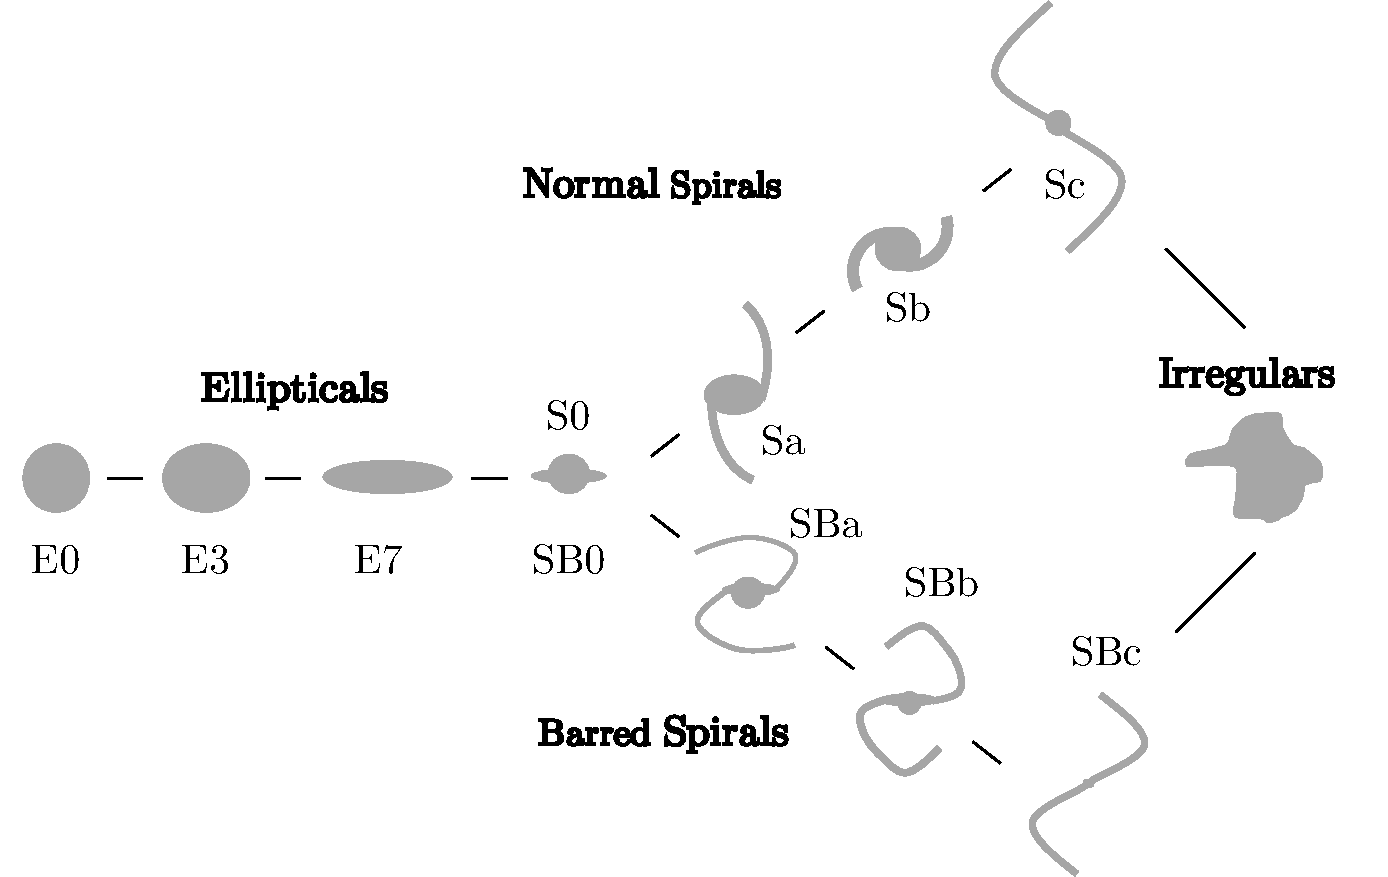
\includegraphics[width=1.0\linewidth]{introduction/hubble_tuning_fork}
\captionof{figure}[Hubble Tuning Fork]{The Hubble Sequence displays the different morphologies of galaxies, they can be classified into three general groups: ellipticals, spirals, and irregulars. The former two can be broken up further, and from the diagram one can see an example pictogram and the respective classification name. \\ (\textit{This diagram has been adapted from An Introduction to Modern Astrophysics} \cite{carroll_astro}.)}
\label{fig:hubble_tuning_fork}
\end{center}

The sequence itself does not show the evolution of the galaxies, rather it provides a way to view the different potential morphologies. It must therefore be asked, what does each grouping from the sequence actually mean? 

Along with the basic classification of appearance the component composition of galaxies can be explored.

Take ellipticals, we see from the Hubble Tuning Fork that they can be described as spherical-like distributions. In fact, they actually range from being virtually spherical (E0) to highly flattened (E7) collections of gas, dust, and dark matter \cite{moore_databook}. Through observation of the stars within them, we find that the majority of them are the older, red coloured variety. This may be due to the fact that early on in the creation of ellipticals, a considerable proportion of the gas went into the formation of stars, thus viewing these galaxies now we find that their stars are predominantly older types \cite{carroll_astro} as new stars are not being born. This could also explain the lack of disks which can be otherwise seen in the spiral galaxies. With not enough material the disk and arms features would not form.

Comparatively, we can describe spiral galaxies as being composed of a central nucleus which has a surrounding disk of material. This disk then has denser regions which can coalesce and form the protruding arms which we can see around the main bulge \cite{carroll_astro}. The later type spirals (Sc and SBc) have arms which are more loosely wound than their earlier types (Sa and SBa) \cite{moore_databook}. With more available gas and dust \cite{carroll_astro}, we would assume that spirals in their various forms would have more opportunities to form new stars than ellipticals. 

It is within the arms of spiral galaxies that we find the creation of new stars. It is within the spiral structure that we find the gravitational field which allows for angular momentum to be transported outwards. Older and less massive stars in the galaxy produce a gravitational field which eventually leads to the shocking of the interstellar gas \cite{binney_galaxies}. As a result the density of the gas in the arms increase and certain regions then collapse to form new young, blue, and massive stars. 

Spiral galaxies therefore have a mix of ages in relation to their stellar population. The arms in a spiral contain young stars whilst the central nucleus is similar to that of elliptical galaxies where the population of stars is composed of older types \cite{carroll_astro, binney_galaxies}.

Irregular galaxies have no noticeable symmetry and no obvious central nucleus, so they do not fall into either of the other two categories.

% TODO from describing the composition of the stars and 'old elliptical stars' we can then go on to discuss the star forming rates and initial mass function
% TODO I should expand on how galaxies can actually be identified from one another

% TODO mention more detail about the two types of spiral galaxies, even in passing - go into more detail about them
% TODO if I am going to discuss galactic formation, should I have mentioned the earlier detail on how ellipticals form stars early on in the galaxies' history? 

% TODO how do I want to write this story? I want a complete picture which is detailed - give some history on the Hubble sequence i.e. Edwin Hubble. 
% TODO I want detail, I need to find the style of writing which I used to have

% what do I really want my narrative to be? 

By knowing these general characteristics, as we continually to improve our observational instruments we can then view deeper into the Universe's past. This means the galactic objects are becoming more and more younger, this is a powerful way for us to build a picture of the evolutionary nature of galaxies and their structure. 

\subsection{Galactic and stellar formation}

% TODO then we can move onto the formation of galaxies, discussing stellar formation rates and the initial mass function
% TODO we want to build up a short but complete picture of what galaxies are 

We introduced the concept that through optical measurements of the stars 

% TODO What do I want to say with this? I want to introduce galaxies, the different types of galaxies, how they form, how they can be confused with other types of structure. 

\subsection{Data} 

askjdnaksld

\subsubsection{HUDF and MUSE}

To obtain spectroscopic information on the Hubble UDF objects, the Multi-Unit Spectroscopic Explorer or MUSE was employed. This instrument is 

% TODO what is MUSE, where it is on the VLT, problems, limitations of MUSE - why it is useful...etc

\onecolumngrid

\begin{figure}
  \begin{subfigure}[b]{0.4\textwidth}
    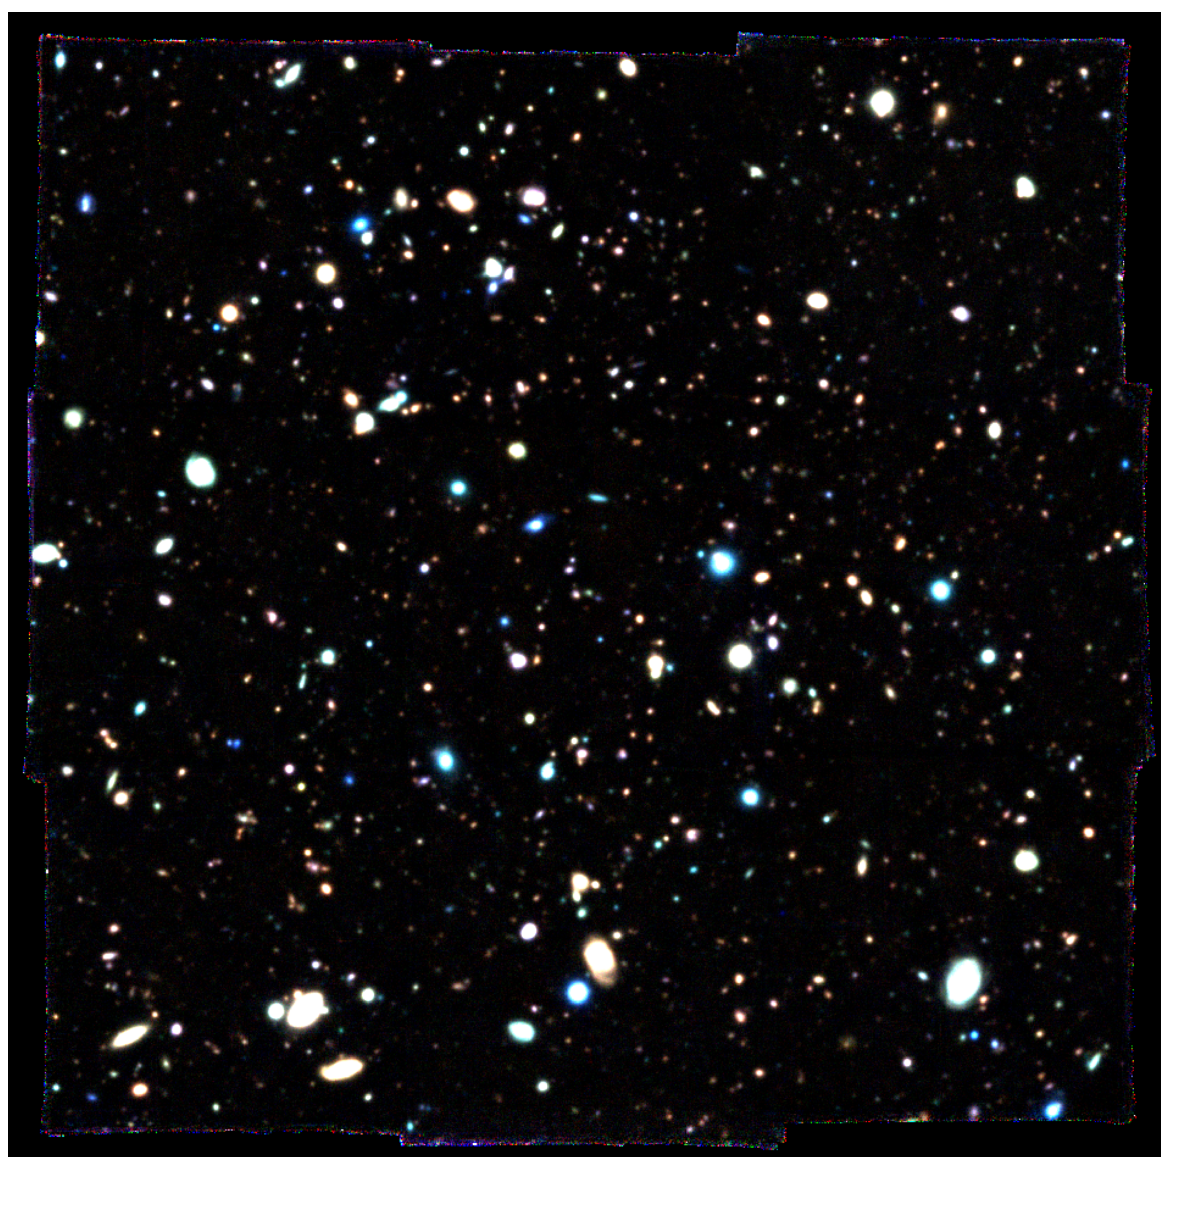
\includegraphics[width=\textwidth]{introduction/muse_colour_image}
    \captionsetup{justification=justified}    
    \caption{MUSE HUDF}               
    \label{fig:muse_colour_image}
  \end{subfigure}
  %
  \begin{subfigure}[b]{0.4\textwidth}
    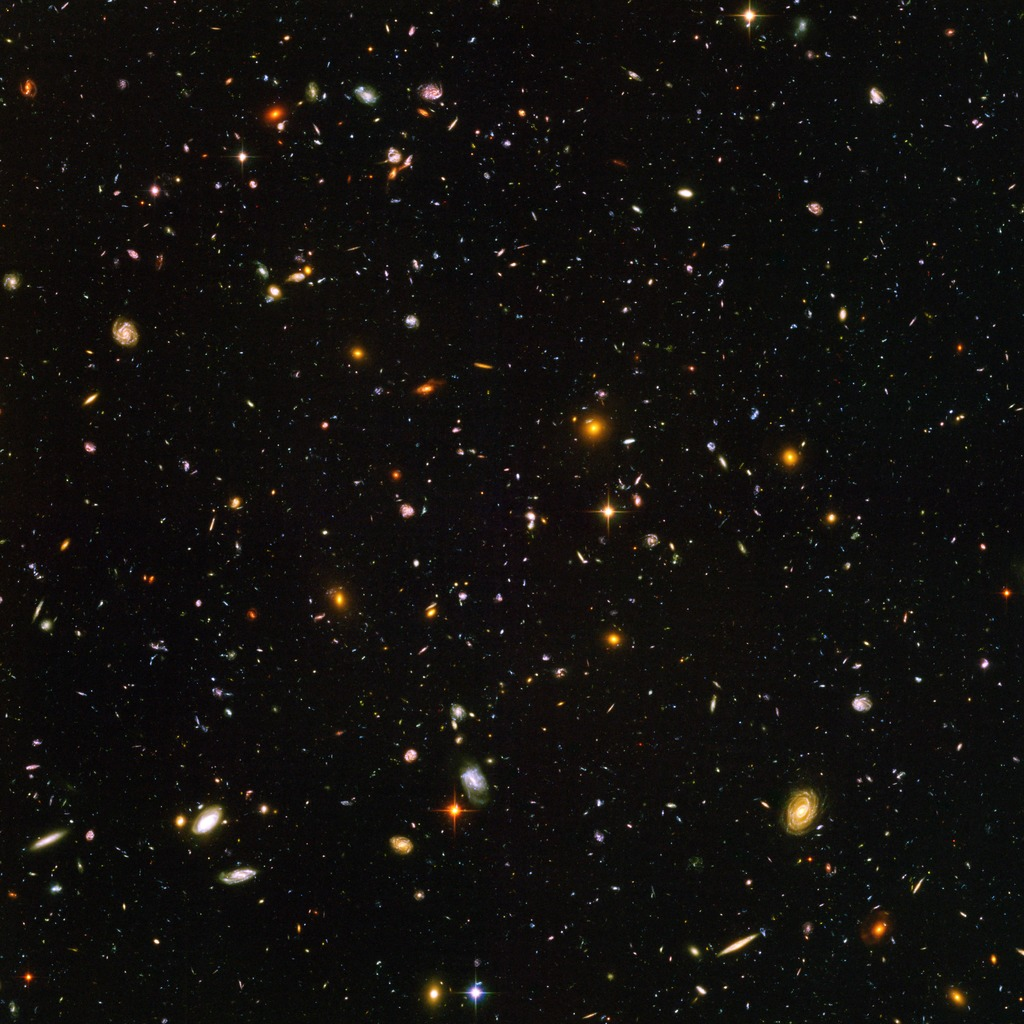
\includegraphics[width=\textwidth]{introduction/hubble_ultra_deep_field}
    \captionsetup{justification=justified}    
    \caption{HST HUDF}
    \label{fig:hubble_ultra_deep_field}
  \end{subfigure}
  \captionsetup{justification=justified}
  \caption[Hubble Ultra Deep Field]{(a) A colour image created from the MUSE spectroscopic data of the HUDF. The wavelength range was split into three equal regions and then collapsed to create three bands (R, G, B). A final colour image was produced by combining these separate frames together. (b) The optical HUDF as captured by the Advanced Camera for Surveys instrument on the Hubble Space Telescope \cite{hudf_image}. }
\end{figure}

\twocolumngrid

asdasd

\subsection{Project Aims}
This paper discusses the study undertaken to understand the dynamics between the gas and stars in galaxies, data extraction is performed on the MUSE data cube, the sample is reduced, doublet fitting performed, applied the data set to a processing package pPXF. 

In section \ref{analysis}, the experimental methods behind the data extraction and analysis are discussed. 

\section{Analysis} 
\label{analysis}

sfsadf

\subsection{Cube extraction}

asdasd

\onecolumngrid

\begin{figure}
  \begin{subfigure}[b]{0.495\textwidth}
    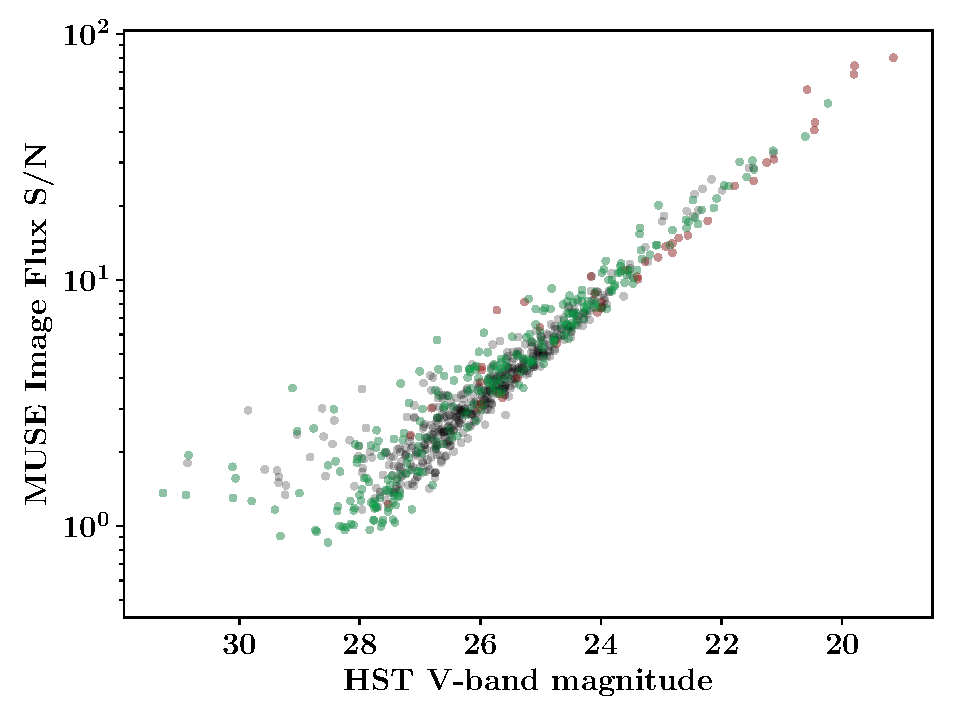
\includegraphics[width=\textwidth]{data/image_sn_vs_vband}
    \captionsetup{justification=justified}
    \caption{Image S/N vs. V-band}
    \label{fig:image_sn_vband}
  \end{subfigure}
  %
  \begin{subfigure}[b]{0.495\textwidth}
    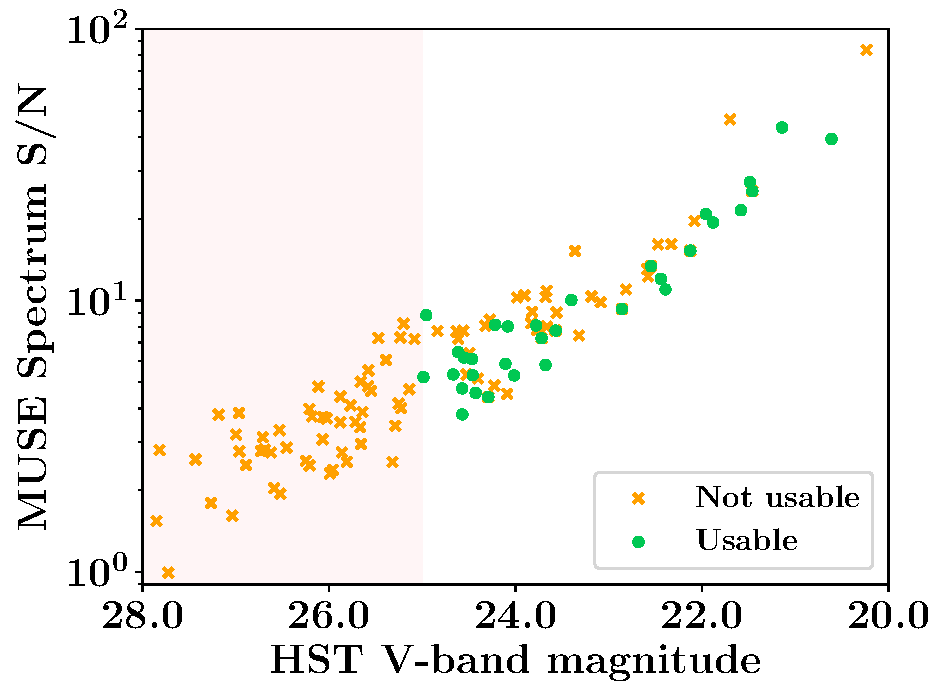
\includegraphics[width=\textwidth]{data/sn_vs_vband}
    \captionsetup{justification=justified}    
    \caption{Spectroscopic S/N vs. V-band}
    \label{fig:spec_sn_vband}
  \end{subfigure}
  \captionsetup{justification=justified}
  \caption[HUDF Objects]{(a) The signal-to-noise of the image flux for every object in the MUSE collapsed image plotted against their respective V-band magnitudes from the HST catalogue. The red points represent those with redshifts $z<0.3$, and the green points are a chosen sample of 300 points as defined by the sextractor probability that they are not stars. (b)}
\end{figure}

\twocolumngrid

asdasd

\begin{center}
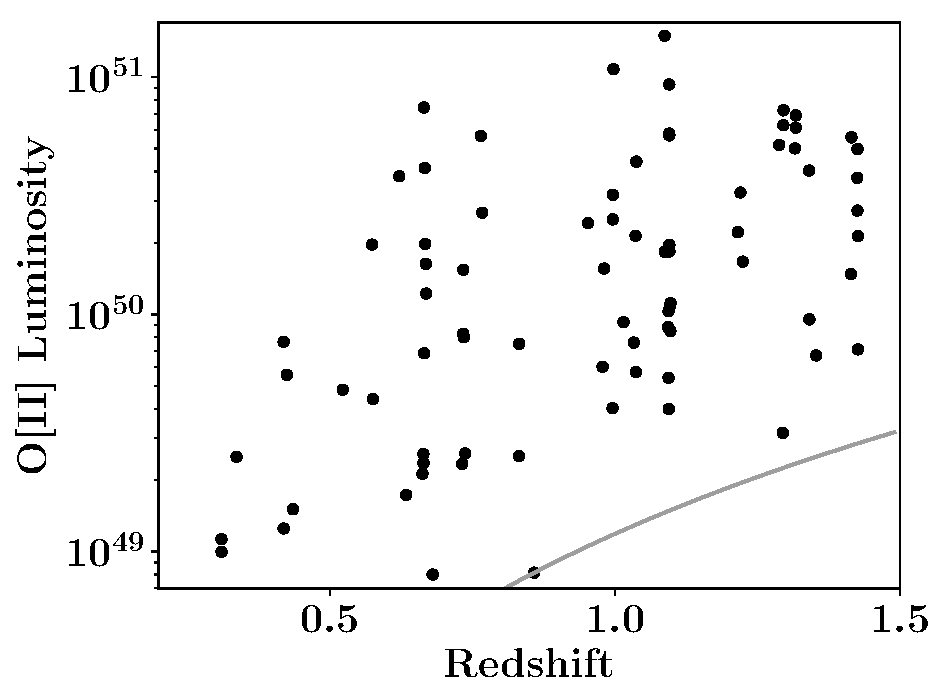
\includegraphics[width=1.0\linewidth]{data/o_ii_luminosity_vs_redshift}
\captionof{figure}[OII Luminosity vs. Redshift]{Graph showing the calculated luminosity for the O[II] doublet plotted against redshift. Data points are plotted as well as a model line representing the lower-limit of the flux from the sample. [???]a}
\label{fig:oiiluminosity_redshift}
\end{center}

aasdasd

\subsection{Line fittings and pPXF} 

After extracting the individual galactic objects from the main MUSE cube, the data had to be verified and then fitted using two different routines: (i) O[II] doublet fitting, and (ii) pPXF absorption line fitting. 

\begin{center}
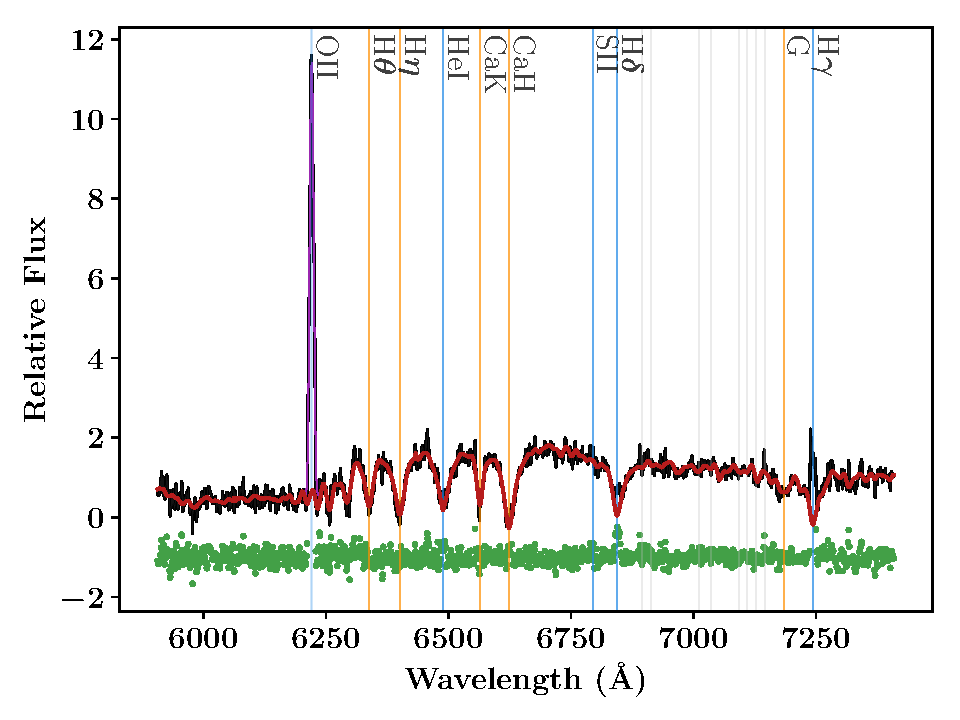
\includegraphics[width=1.0\linewidth]{data/cube_1804_fitted}
\captionof{figure}[OII Luminosity vs. Redshift]{Fitting of a galaxy spectrum with pPXF.}
\label{fig:oiiluminosity_redshift}
\end{center}

\begin{center}
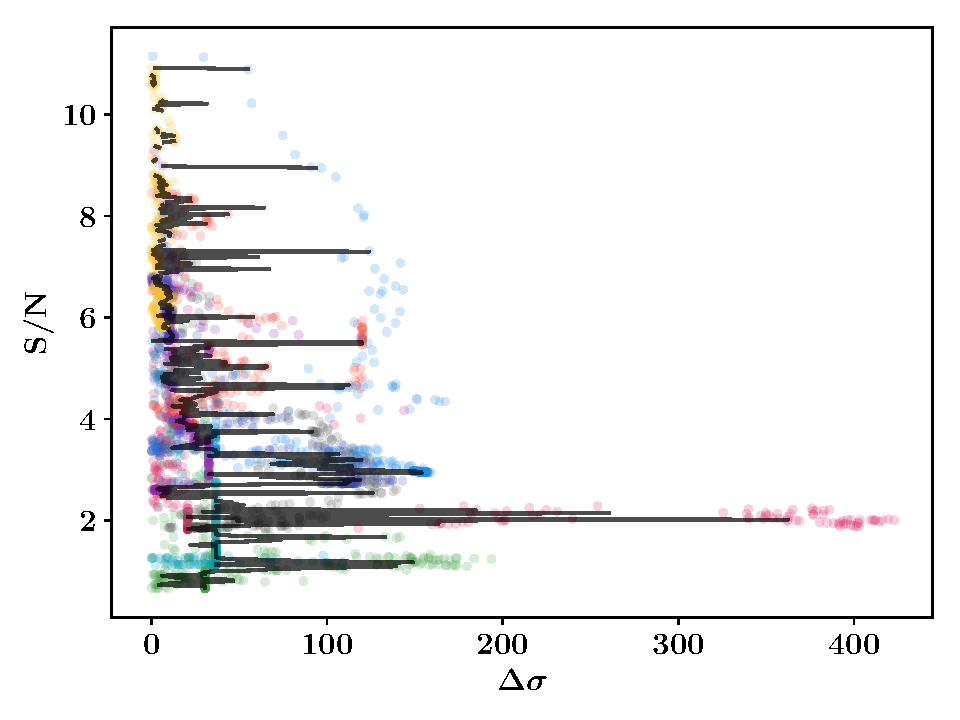
\includegraphics[width=1.0\linewidth]{data/reprocessed_sn_vs_delta_sigma}
\captionof{figure}[S/N vs. delta(sigma)]{The signal-to-noise versus the fractional error of the $\sigma$ line width of the pPXF curve fittings.}
\label{fig:oiiluminosity_redshift}
\end{center}

\section{Discussion} 

-

\section{Conclusions}
 
In conclusion, through extensive data and statistical analysis it can be said that the dynamics of stars and gas in galaxies are ... (?) 

\begin{acknowledgments}
The author would like to thank Dr.~M.~Swinbank and Alfie Tiley for their continual help and support throughout the project period, without which, the project would have been experimentally grounded.
\end{acknowledgments}

\bibliographystyle{unsrt}
\bibliography{stars_gas_dynamics}

\end{document}
